\documentclass{article}
\usepackage{spconf,amsmath,graphicx}
\usepackage{amssymb,mathtools}
\usepackage{graphicx}
\usepackage{listings}
\usepackage{url}
\usepackage{hyperref}
\graphicspath{ {./images/} }
\DeclarePairedDelimiter{\norm}{\lVert}{\rVert}
\DeclarePairedDelimiter{\abs}{\lvert}{\rvert}
\def\x{{\mathbf x}}
\def\L{{\cal L}}
\title{Page Ranking Algorithim}
%
% Single address.
% ---------------
\name{Suresh (M20AIE313), Utkarsh (M20AIE318), Pradeep (M20AIE275)}
\address{IIT Jodhpur}
\begin{document}
%\ninept
%
\maketitle
%
\begin{abstract}
    In a real-world scenario a web surfer searches a page over the internet in a million of pages and search engines needs to analyse the given input and identify the all-matching web pages for the user input. 
    In order to ensure search engine recommending the right page The algo should measures the importance of each page. 
    Page Ranking is a metric which we used as a importance metric while filtering the content and recommend any page. \vspace{2cm}
\end{abstract}
%
\begin{keywords}
PageRanking, Web Crawling, World Wide Web, Search Engine
\end{keywords}
%

\section{Introduction}
\label{sec:intro}
World Wide Web has grown exponentially over the years and with the introduction of search engines like google, bing, aol etc we have seen a record breaking increase in web searches. While every search engine uses a certain specific underline algorithm to provide the best pages for a given query, here we are trying to find some of the basic solutions to this problem presented in \href{http://ilpubs.stanford.edu:8090/422/1/1999-66.pdf}{paper} . With this project we have created a demo where we can crawl a certain page and provide ranking to each of the page based on the various factors. The common factors include:
\begin{itemize}
    \item Initial PageRank for any page will be $\frac{1}{Total Node Count}$
    \item Computing the value of PageRank based on number of web links current page can be reached from.
    \item Uniform distribution of page rank between various pages under same parent.
    \item Included dampling factor which helps in finding probability of user clicking on the current page links randomly.
\end{itemize}

We have tried to go through various articles apart from this papaer which are realted to web crawling to identify how we can crawl a specific web page.

\section{Related Works}
\label{sec:relWork}
\begin{itemize}
    \item \href{http://ilpubs.stanford.edu:8090/422/1/1999-66.pdf}{Actual Paper} 
    \item \href{https://en.wikipedia.org/wiki/PageRank}{PageRank wikipedia} 
    \item \href{https://www.webfx.com/blog/internet/what-is-a-web-crawler/#:~:text=For%20example%2C%20Google%20has%20its,DuckDuckBot%20for%20DuckDuckGo}{Web Crawler} 
\end{itemize}

\section{Definitions}
\label{sec:def}

\begin{itemize}
    \item \textbf{PageRank (PR)} is an algorithm used by search engines to rank websites in their search engine results measuring the importance of website pages. The algorithims returns a number between 0 and 1. The term was first coined in Google after one of its founders Larry Page. The number actually represent the likelihood that a person randomly clicking on links will arrive at any particular page.
    \item \textbf{Damping factor} The random surfer on the internet will always end up with the dangling node (having no edges) and given any point in time the dampling factor carried is $d$. The probability of surfer choosing the random next link is $d$ and We assumed $d=0.85$ and 0.15\% shared in each iteration and total PR values of all n nodes is 1. This will prevent the convergence of value 0 or 1.
    \item \textbf{Convergence property} page rank iteratively computed until norm distance $\delta \leftarrow \norm{R_{i+1} - R_i}_1$ is reaching the closer value to have the precision. We can control the page rank precision with the precision value we given. We assumed it to be from anywhere between 10e-5 to 10e-10. In other words, the computation ends for each page when some small $ \abs{R_{t+1} - R_t} < \epsilon$
    \item \textbf{Dangling Node} A node which has no outDegree is a dangling node.
    \item \textbf{Dangling Rank} Rank of a dangling node is called dangling rank.
\end{itemize}

\newpage

\section{Implementation}
\label{sec:space}
To compute PageRank we are iteratively computing the page until we meet the precision factor.

\subsection{Computing Page Rank}
\label{sec:computing-page-rank}
To compute PageRank, Let $S$ be almost any vector over WebPages ex. $E$. We can use below formulae to compute PageRank. $\epsilon$ is precision factor and $\delta$ is normalization factor

\begin{equation}
    \begin{align*}
        R_0 \leftarrow S\\
        & loop:\\
            & & R_{i+1} \leftarrow AR_i\\
            & & d \leftarrow \norm{R_i}_1 - \norm{R_{i+1}}_1\\
            & & R_{i+1} \leftarrow R_{i+1} + dE\\
            & & \delta \leftarrow \norm{R_{i+1} - R_{i}}_1\\
        & while(\delta > \epsilon) 
    \end{align*}
\end{equation}

\subsection{Basic formulae to compute page rank}
\label{sec:computing-page-rank}
\begin{equation}
    PR(p_i) = \frac{1-d}{N} + d \sum_{p_j \epsilon M(p_i)} \frac{PR(p_j)}{L(p_j)}
\end{equation}

\subsection{Code Blocks}
\begin{lstlisting}[language=Java]
    //Equation(2) is represented in code as below
    ranks.add(((1 - df) / graph.getNodeCount()) 
            + df * sum);
	danglingRank = computeDanglingRank(danglingRank, outDegree,
             node.getNumber("page_rank"));

    //Equation(1) is represented in code as below
    normDistance += Math.abs(
                (ranks.get(i) + danglingRank) - 
                graph.getNode(i).getNumber("page_rank"));
\end{lstlisting} 

\newpage
.
\newpage
\subsection{Graph Code with actual crawled data}

\subsubsection[Crawled Graph - Nodes]{Crawled Graph - Nodes}
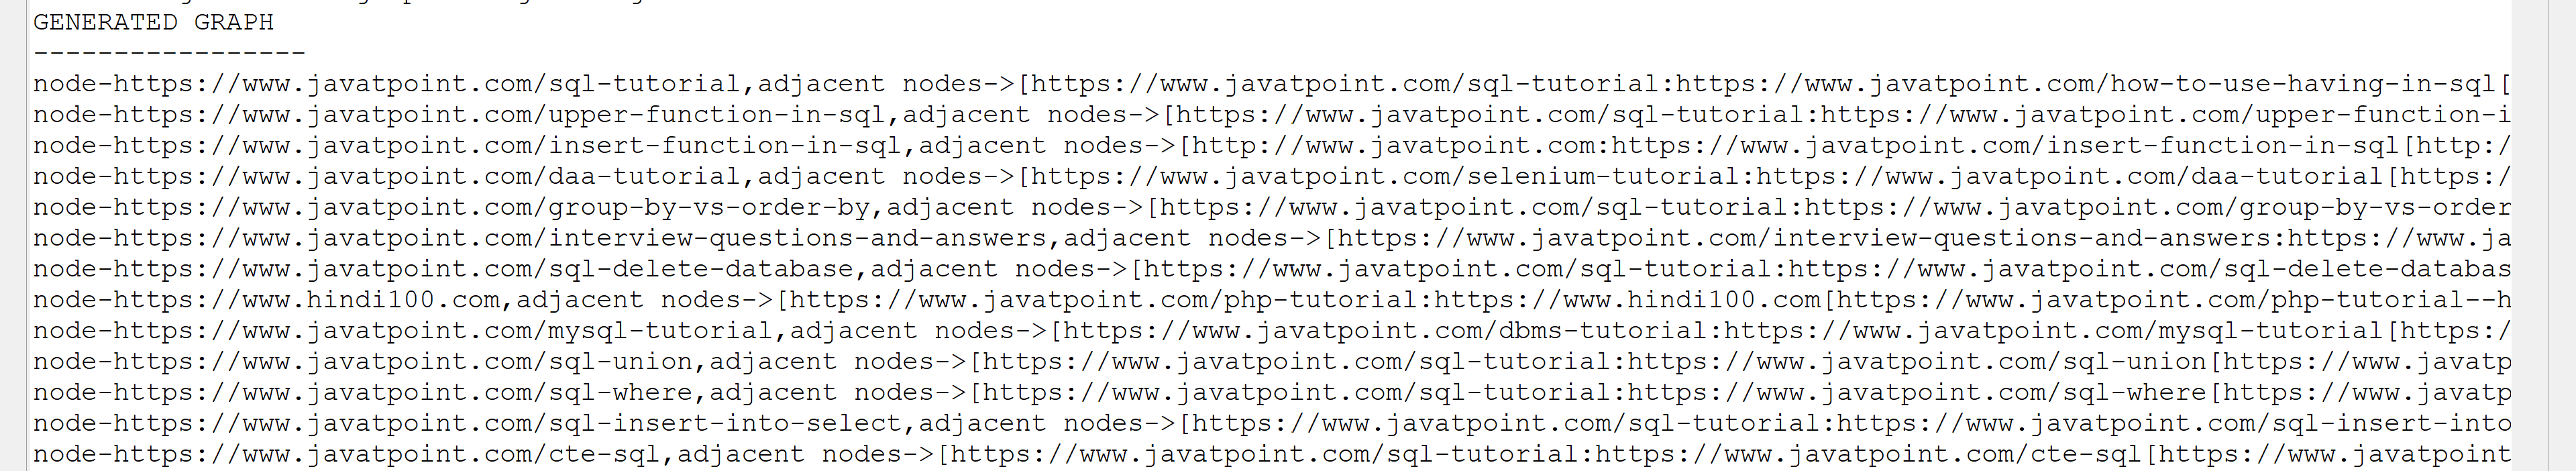
\includegraphics[scale=0.06]{image1.png}

\subsubsection[Crawled Graph - Edges]{Crawled Graph - Edges}
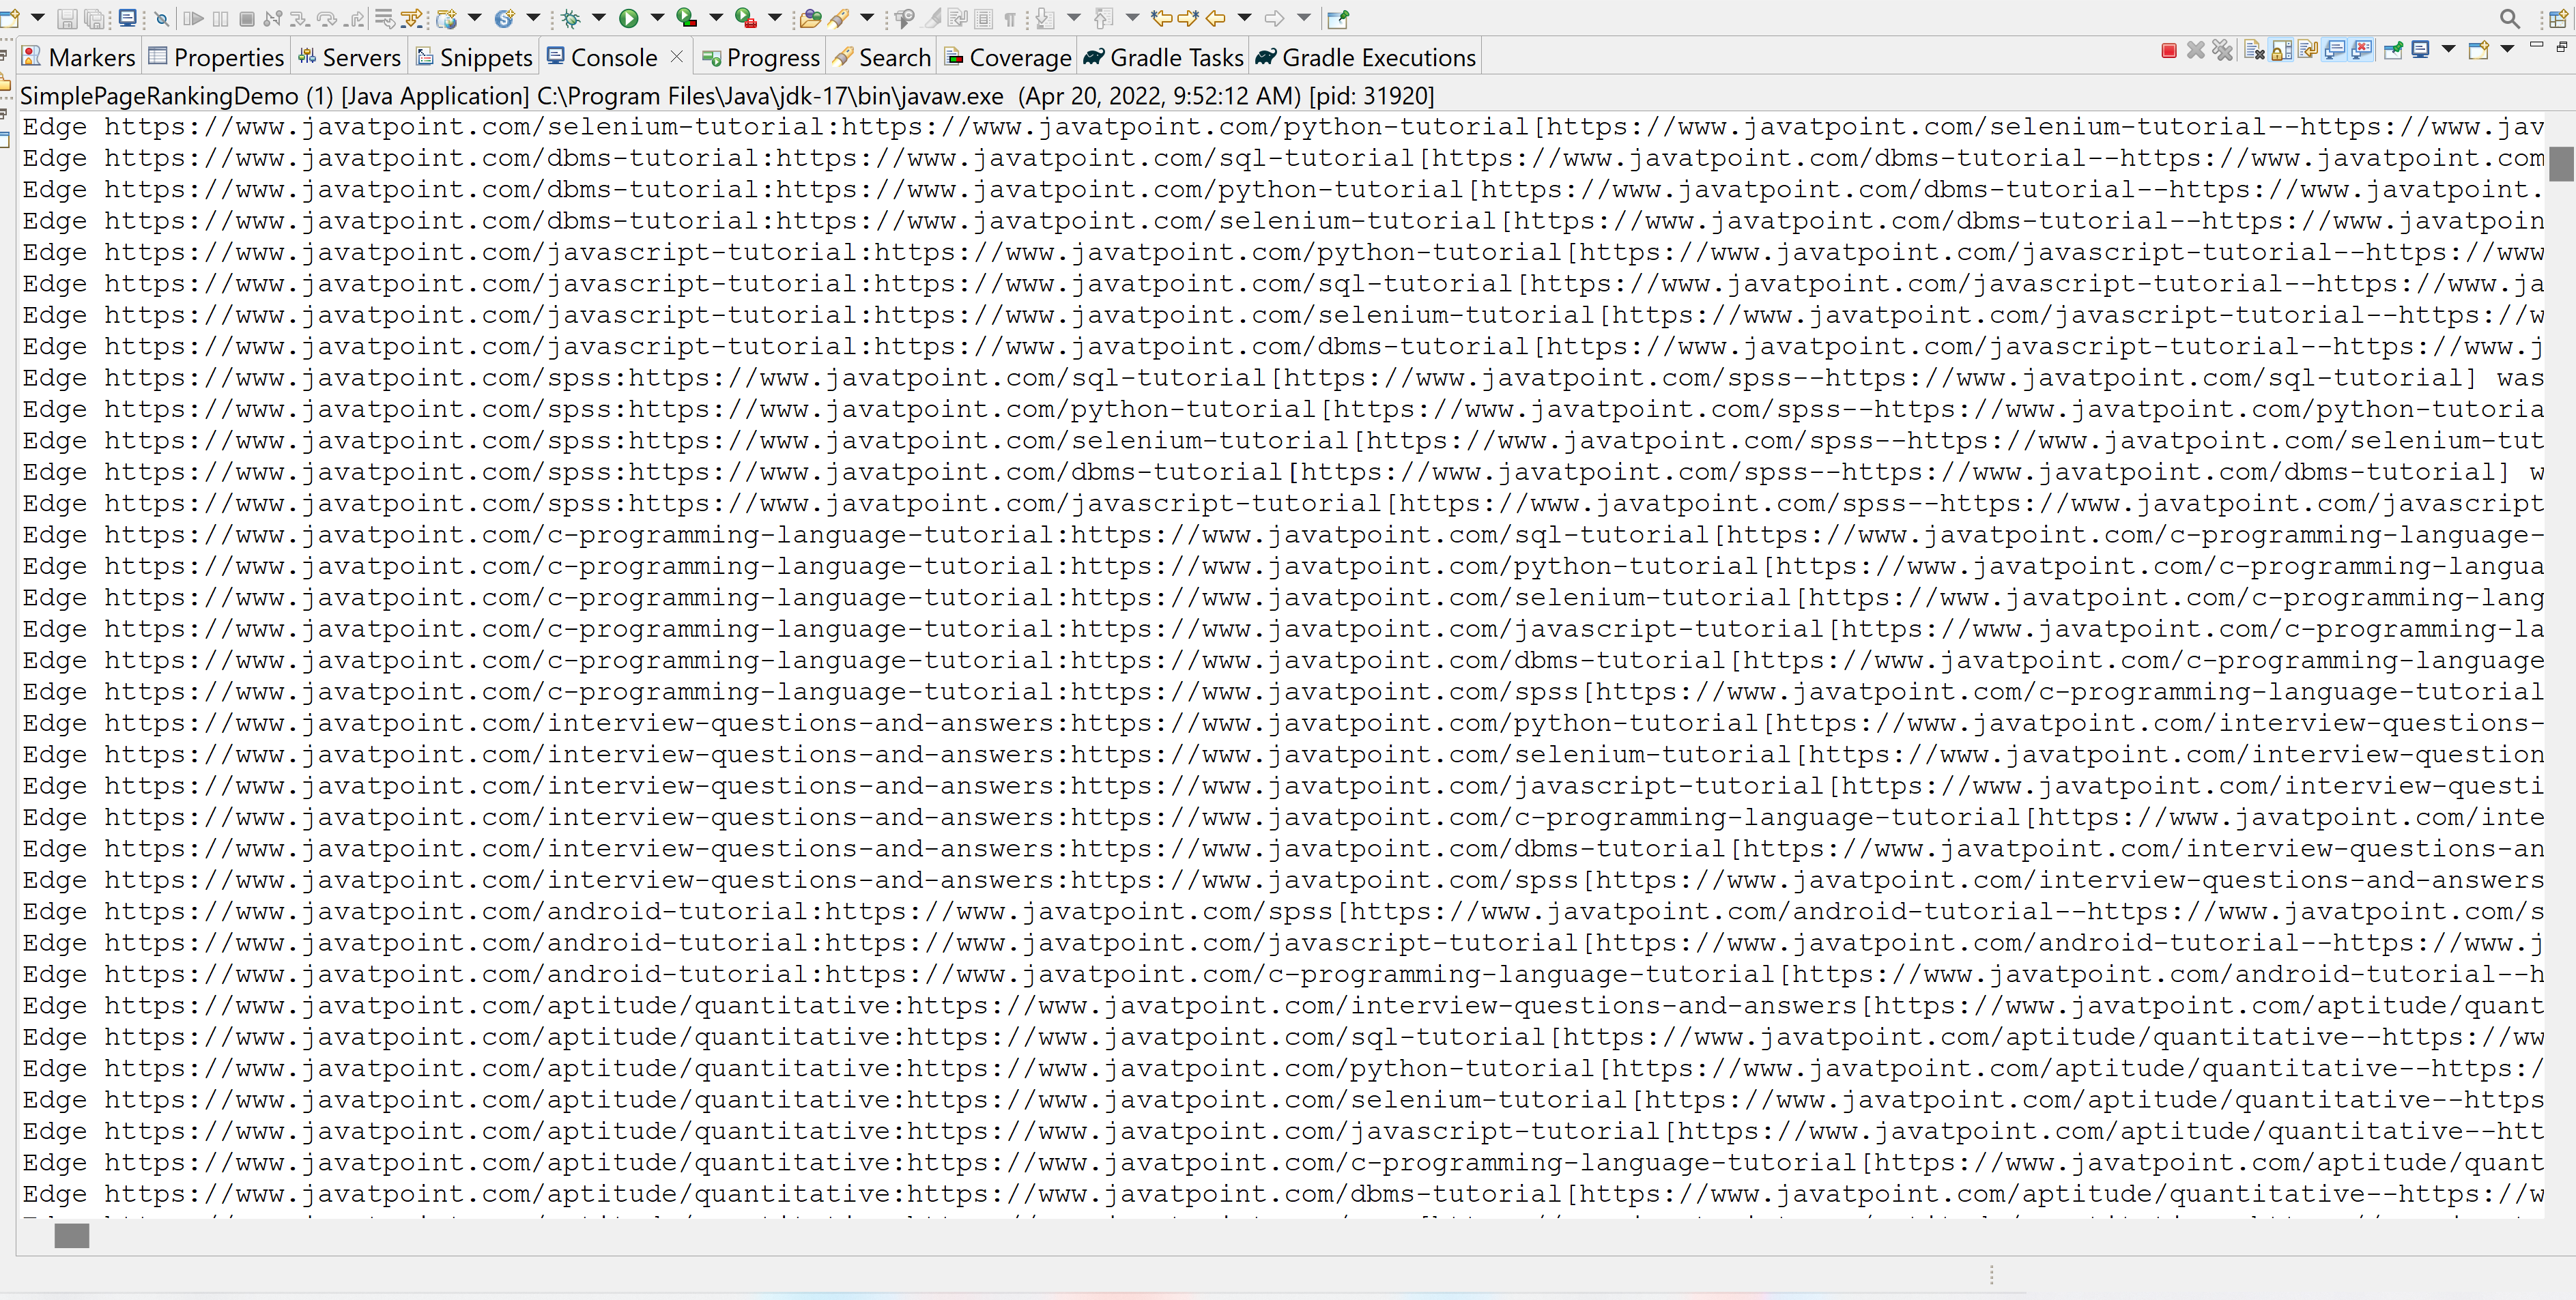
\includegraphics[scale=0.06]{image2.png}

\subsubsection[Output ranks in each iteration]{Output ranks in each iteration}
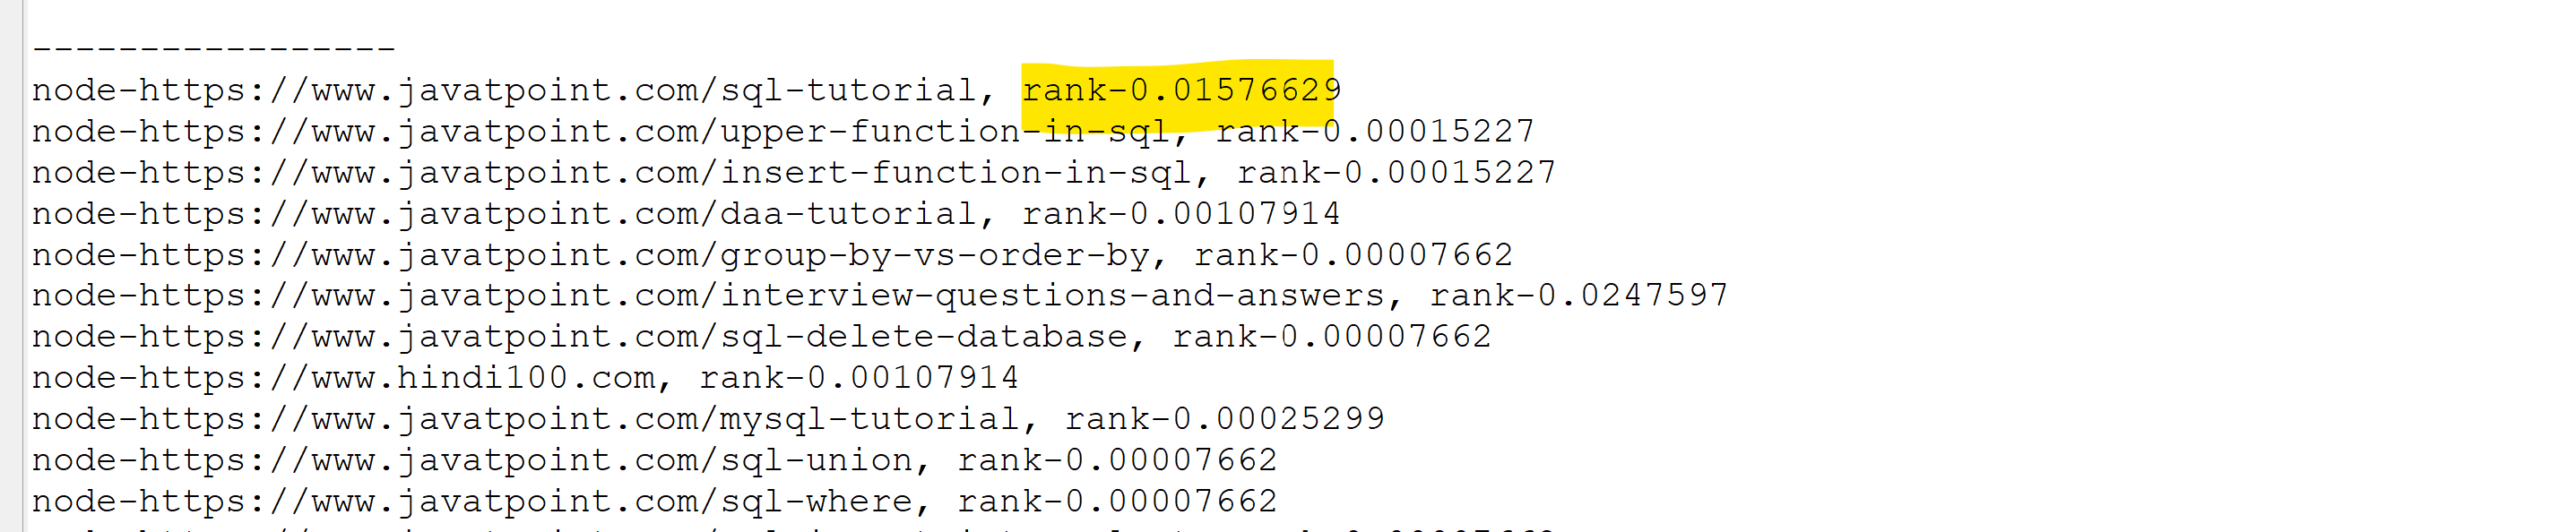
\includegraphics[scale=0.1]{image3.png}

\subsubsection[Finalized Output ranks]{Finalized Output ranks}
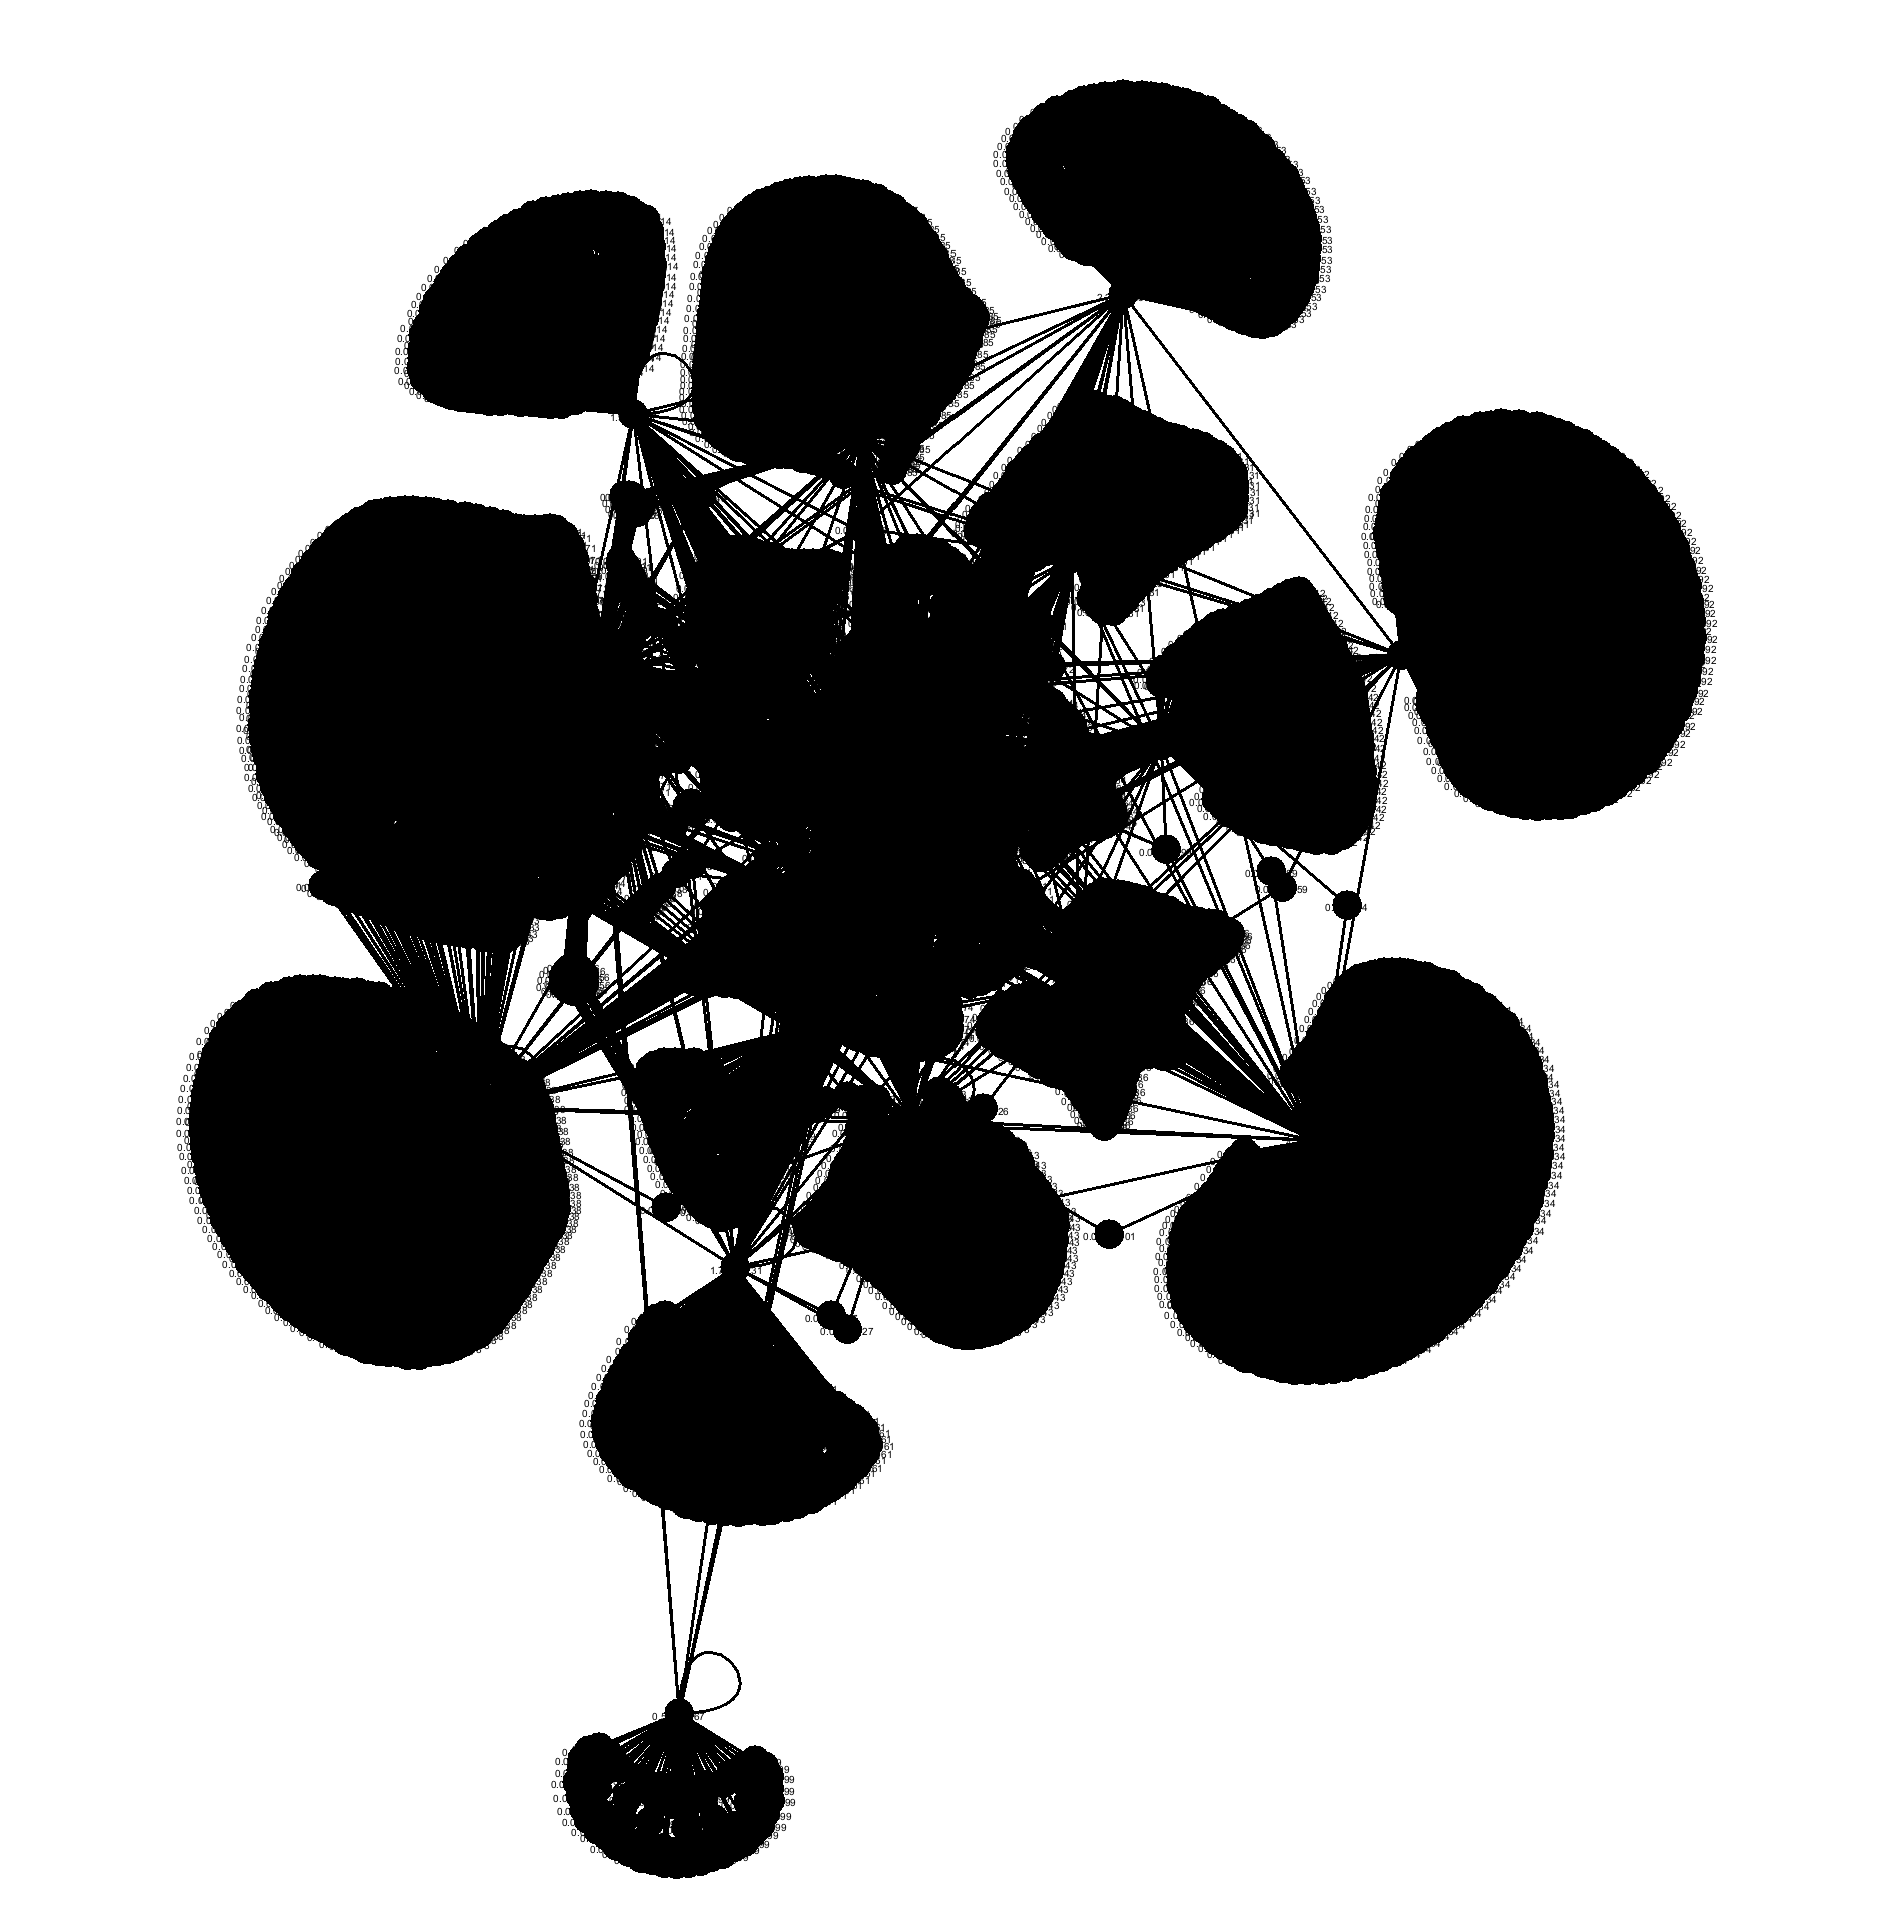
\includegraphics[scale=0.1]{image4.png}

\newpage

\section{Summary}
\label{sec:summary}
In this project we have successfully crawled a web page, extarcted links from that webpage, and then provided PageRank to each of the extracted link based on the PageRank algorithim.


\bibliographystyle{IEEEbib}
\bibliography{strings,refs}

\end{document}
